\section{Wie kann der Begriff Kraftwerksreserve definiert werden?}

	Da der Begriff Kraftwerksreserve nicht genau definiert ist, wird im Folgenden auf die unterschiedlichen Arten der Kraftwerksreserven eingegangen.
	Grundlage bildet der Strommarkt, welcher in Kapitel \ref{sect: Wie funktioniert der deutsche Strommarkt?} behandelt wird.
	Aufgrund der Folgen des Ukrainekonflikts ist ebenfalls eine weitere Art der Reserve hinzugekommen.

	\subsection{Wie funktioniert der deutsche Strommarkt?} \label{sect: Wie funktioniert der deutsche Strommarkt?}
	
		In Deutschland gibt es einen Energy-Only-Market (EOM).
		Dies bedeutet, dass ausschließlich der tatsächlich produzierte Strom gehandelt wird.
		Anders wäre dies bei dem viel diskutierten Kapazitätsmarkt, indem auch vorgehaltene Leistungen für z.B. Dunkelflauten vergütet werden (haucap).
		Die Preisbildung folgt dem Prinizip der Marit-Order (s. Abb. \ref{Abb. Strompreisbildung Merit Order}).
		In der Merit-Order werden alle Stromproduzenten, welche zu gegebenen Zeitpunkt ihren Strom am Markt anbieten, nach ihren jeweiligen Grenzkosten aufsteigend aufgelistet.
		Der Stromerzeuger mit den geringsten Grenzkosten, darf als erstes einspeisen und nach ihm derjenige mit den nächst größeren Grenzkosten.
		Als Grenzkosten werden die Erzeugungskosten für die auf dem Markt genau angebotene Strommenge bezeichnet.
		Der Stromproduzent, welcher mit seiner angebotenen Strommenge Angebot und Nachfrage deckt, legt den zu vergütenen Strompreis für alle anderen Marktteilnehmer in der Merit-Order unter ihm fest.
		Dieses Kraftwerk heißt Grenzkostenkraftwerk.
		In Abbildung \ref{Abb. Strompreisbildung Merit Order} ist die Reihenfolge der Stromerzeugungsart und den typisch zu erwartenden Grenzkosten dargestellt. \\
		
		\begin{figure} [H]
			\centering
			\label{Abb. Strompreisbildung Merit Order}
			\includegraphics[page=82,trim=140 282 130 375, clip, width=\textwidth]{./anhang/Doktorarbeit Reitsam.pdf}
			\caption{Strompreisbildung an der Börse nach dem Merit-Order-Prinzip \cite{Doktorarbeit_Reitsam}}
		\end{figure}
		
		In der Merit-Order weist die Stromerzeugung aus erneuerbaren Energien Grenzkosten von nahezu Null auf.
		Die Folge des Ausbaus von erneuerbaren Energien ist, dass konventionelle Kraftwerke mit hohen Grenzkosten, vor allem Gas- und Ölkraftwerke, in der Reihenfolge nach rechts gerückt werden (Merit-Order-Effekt, s. Abb. \ref{Abb. Strompreisbildung Merit Order}).
		Das Verdängen der Gas-,Öl- sowie Pumpspeicherkraftwerke führen zu einem sinkenden Strompreis an der Böse \cite{Frauenhofer_PV_Bericht}.
		Dadurch sind diese Kraftwerke nur bei mangelndem Wind und mangelnder Sonneneinstrahlung an der Stromproduktion beteiligt.
		Für den Strompreis bedeutet dies teilweise erhebliche Schwankungen je nach aktueller Wetterlage und geringe bzw. unvorhersehbare Betriebsstunden der gennanten Kraftwerke. 
		Damit werden die Anreize gut und schnell regelbare Gaskraftwerke zu errichten und wirtschaftlich betreiben zu können deutlich eingedämmt, obwohl die Kraftwerksleistung ohne Vergütung vorgehalten wird \cite{Frauenhofer_PV_Bericht}.
		Gegensätzlich dazu verlangt der Ausbau regenerativer Stromerzeuger einen Zuwachs gut und schnell regelbarer Gaskraftwerke \cite{Doktorarbeit_Reitsam}. \\
		
		Die Forderung eines Kapazitätsmarkts, indem auch vorgehaltene Kraftwerksleistung bepreist wird, gewinnt dahingehend an Bedeutung.
		Den Karftwerksbetriebern fällt es zunehmend schwer ihre konventionellen Kraftwerke aufgrund der bereits erörterten fehlenden Betriebsstunden rentabel zu betreiben.
		Auch ohne weiteren Ausbau von erneuerbaren Energien wird bei Dunkelflauten gerade in den wenig sonnigen Wintermonaten Janaur und Februar weiterhin Residuallast gebraucht.
		Konträr dazu wurde in der EEG-Nobelle aus dem jahr 2014 eine strategische Kraftwerksreserve aus Braunkohlekraftwerken entschieden (BMWi).		
				
	\subsection{Kraftwerksreserven zur Netzfrequenzstabilisierung}
	
		\begin{wrapfigure}{r}{0.5\textwidth}
			\centering
			\includegraphics[page=92,trim=250 71 50 450, clip, width=0.5\textwidth]{./anhang/Elektrizitätswirtschaft.pdf}
			\caption{Regelzonen und Übertragungsnetzbetreiber in Deutschland \cite{Elektrizitätswirtschaft}}
			\label{Abb. Regelzonen Deutschland}
		\end{wrapfigure}
	
		Die Kraftwerksreserven zur Netzfrequenzstabilisierung fallen unter den Begriff des Regelenergiemarkts.
		Aufgrund des liberalisierten Strommarkts besitzen die Übertragunsnetzbetreiber keine eigenen Kraftwerke, sodass für die Stabilisierung Verträge mit Energieversorgungsunternehmen (EVU) geschlossen werden müssen. \\
			
		Unter Regelenergie versteht man zum einen die Reservierung von Kraftwerksreserven bzw. -kapazitäten (Regelleistung) und zum anderen den Ausgleich von Regelzonenungleichgewichten (Regelarbeit) \cite{Elektrizitätswirtschaft}.
		Da es im Stromnetz zu negativen und positiven Abweichungen der Frequenz kommen kann, wird zur Kompensation sowohl positive und negative Regelarbeit benötigt.
		Anders als bei der Regelleistung wird eine gelieferte Strommenge in \si{\mega\watt\hour} vergütet.
		Um Unterschiede zwischen Angebot und Nachfrage unter den vier deutschen Regelzonen zu decken, wird eine Reservierung von Kraftwerksreserven erforderlich (Regelzonen s. Abb. \ref{Abb. Regelzonen Deutschland}). 
		In diesem Fall erfolgt eine Bezahlung der Kraftwerke unabhängig von der gelieferten Strommenge und Einsatzzeit \cite{Elektrizitätswirtschaft}. 
		Die Bezahlung ist als eine Art Entschädigung für das Vorhalten von Kraftwerkskapazitäten, gegebenenfalls nicht Abrufen und den damit verbundenen Fixkosten der Einsatzbereitschaft zu verstehen.   \\
		
		\begin{figure} [H]
			\centering
			\label{Abb. Beispielhafte Darstellung der Regelenergie in Abhängigkeit der Netzfrequenz}
			\includegraphics[page=115,trim=50 80 50 470, clip, width=\textwidth]{./anhang/Elektrizitätswirtschaft.pdf}
			\caption{Beispielhafte Darstellung der Regelarbeit in Abhängigkeit der Netzfrequenz \cite{Elektrizitätswirtschaft}}
		\end{figure}
		
		
	
	\subsection{Kraftwerksreserven zur Reserveleistungsvorhaltung}